%\documentstyle[epsf,twocolumn]{jarticle}       %LaTeX2e仕様
\documentclass[twocolumn]{jarticle}     %pLaTeX2e仕様(platex.exeの場合)
% \documentclass[onecolumn]{ujarticle}   %pLaTeX2e仕様(uplatex.exeの場合)
%%%%%%%%%%%%%%%%%%%%%%%%%%%%%%%%%%%%%%%%%%%%%%%%%%%%%%%%%%%%%%
%%
%%  基本バージョン
%%
%%%%%%%%%%%%%%%%%%%%%%%%%%%%%%%%%%%%%%%%%%%%%%%%%%%%%%%%%%%%%%%%
\setlength{\topmargin}{-45pt}
%\setlength{\oddsidemargin}{0cm}
\setlength{\oddsidemargin}{-7.5mm}
%\setlength{\evensidemargin}{0cm}
\setlength{\textheight}{24.1cm}
%setlength{\textheight}{25cm}
\setlength{\textwidth}{17.4cm}
%\setlength{\textwidth}{172mm}
\setlength{\columnsep}{11mm}

%\kanjiskip=.07zw plus.5pt minus.5pt


% 【節が変わるごとに (1.1)(1.2) … (2.1)(2.2) と数式番号をつけるとき】
%\makeatletter
%\renewcommand{\theequation}{%
%\thesection.\arabic{equation}} %\@addtoreset{equation}{section}
%\makeatother

%\renewcommand{\arraystretch}{0.95} 行間の設定
%%%%%%%%%%%%%%%%%%%%%%%%%%%%%%%%%%%%%%%%%%%%%%%%%%%%%%%%
%\usepackage{graphicx}   %pLaTeX2e仕様(\documentstyle ->\documentclass)
\usepackage[dvipdfmx]{graphicx}
\usepackage{subcaption}
\usepackage{multirow}
\usepackage{amsmath}
\usepackage{url}
\usepackage{ulem}
\usepackage{algorithm}
\usepackage{algorithmic}
\usepackage{listings} %,jlisting} %日本語のコメントアウトをする場合jlistingが必要
%ここからソースコードの表示に関する設定
\lstset{
  basicstyle={\ttfamily},
  identifierstyle={\small},
  commentstyle={\smallitshape},
  keywordstyle={\small\bfseries},
  ndkeywordstyle={\small},
  stringstyle={\small\ttfamily},
  frame={tb},
  breaklines=true,
  columns=[l]{fullflexible},
  numbers=left,
  xrightmargin=0zw,
  xleftmargin=3zw,
  numberstyle={\scriptsize},
  stepnumber=1,
  numbersep=1zw,
  lineskip=-0.5ex
}
%%%%%%%%%%%%%%%%%%%%%%%%%%%%%%%%%%%%%%%%%%%%%%%%%%%%%%%%
\begin{document}

	%bibtex用の設定
	%\bibliographystyle{ujarticle}

	\twocolumn[
		\noindent
		\hspace{1em}
		2020 年 11 月 6 日
		ゼミ資料
		\hfill
		B4 杉山 竜弥
		\vspace{2mm}

		\hrule
		\begin{center}
			{\Large \bf 進捗報告}
		\end{center}
		\hrule
		\vspace{9mm}
	]

\section{今週やったこと}
\begin{itemize}
  \item 閾値によるアーキテクチャの評価実験
  \item 猫データセットへの適用
\end{itemize}

\section{実験}

前回までの結果(A)に加え, 閾値によるアーキテクチャ決定をした場合(B)の性能評価を行った.

\begin{table}[tb]
  \begin{center}
    \caption{実験の設定}
    \begin{tabular}{|c|c|} \hline
      base model & VGG19 \\ \hline
      Optim($w$) & SGD(lr=0.0090131, momentum=0.9) \\ \hline
      % Optim($\alpha$) & Adam(lr=0.005, $\beta$=(0.5, 0.999)) \\ \hline
      Scheduler($w$) & Step($\gamma$=0.2344, stepsize=100) \\ \hline
      Loss & Cross Entropy Loss \\ \hline
      dataset & cifar10 \\ \hline
      batch size & 64 \\ \hline
      epoch & 150 \\ \hline
    \end{tabular}
    \label{tab:setting}
  \end{center}
\end{table}

表\ref{tab:setting}に評価時の実験設定を示した.

\subsection{結果}

% 評価時のグラフは./graphを参照.
表\ref{tab:accg}にはテスト精度の結果を示した.
A, Bでは探索結果の$\alpha$が同じ条件で, 手法の違いを比較した.

図\ref{fig:param}, \ref{fig:short}にはパラメータ数, ショートカット数に対するそれぞれの精度を図示した.
この結果から150 epoch時点で, 2つの手法で性能はともに下がっているため手法に拠らず, 探索の結果の$\alpha$自体が悪くなっている可能性が高い.
また手法Bでは性能は劣るものの, アーキテクチャのスケールに対して効率の良い精度が得られていることが分かった. 手法Aがより優れた性能であるのは, 単にパラメータ数が多いからであると思われる.

\begin{table*}[t]
  \begin{center}
    \caption{各アーキテクチャの精度}
    \begin{tabular}{|c|c|c|c|c|}
    \hline
    \multicolumn{2}{|c|}{architecture} & \textbf{\begin{tabular}[c]{@{}c@{}}test accuracy\\ (\%)\end{tabular}} & \textbf{\begin{tabular}[c]{@{}c@{}}param\\ (M)\end{tabular}} & \textbf{\begin{tabular}[c]{@{}c@{}}number of\\ shortcuts\end{tabular}} \\ \hline
    \multirow{3}{*}{\begin{tabular}[c]{@{}c@{}}architecture\\ A\end{tabular}} & 50 epoch & 93.70 $\pm$ 0.22 & 21.06 $\pm$ 0.07 & 12.7 $\pm$ 1.4 \\ \cline{2-5}
     & 100 epoch & 94.02 $\pm$ 0.12 & 21.50 $\pm$ 0.11 & 18.2 $\pm$ 0.9 \\ \cline{2-5}
     & 150 epoch & 93.90 $\pm$ 0.17 & 21.57 $\pm$ 0.25 & 18.9 $\pm$ 0.6 \\ \hline
     \multirow{3}{*}{\begin{tabular}[c]{@{}c@{}}architecture\\ B\end{tabular}} & 50 epoch & 93.57 $\pm$ 0.19 & 20.45 $\pm$ 0.09 & 5.8 $\pm$ 1.2 \\ \cline{2-5}
      & 100 epoch & 93.93 $\pm$ 0.08 & 20.73 $\pm$ 0.10 & 9.8 $\pm$ 1.0 \\ \cline{2-5}
      & 150 epoch & 93.92 $\pm$ 0.12 & 20.76 $\pm$ 0.15 & 10.6 $\pm$ 1.0 \\ \hline
    \multicolumn{2}{|c|}{random architect} & 93.60 $\pm$ 0.15 & 21.50 $\pm$ 0.23 & 12.7 $\pm$ 1.4 \\ \hline
    \multicolumn{2}{|c|}{baseline (VGG19)} & 93.03 $\pm$ 0.10 & 20.04 & 0 \\ \hline
    \end{tabular}
    \label{tab:accg}
  \end{center}
\end{table*}

\begin{figure*}[tb]
 \begin{minipage}{0.5\hsize}
 	\begin{center}
 		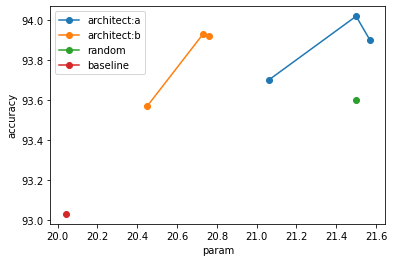
\includegraphics[clip,width=75mm]{param.png}
 		\caption{パラメータ数に対する精度}
 		\label{fig:param}
 	\end{center}
 \end{minipage}
 \begin{minipage}{0.5\hsize}
 	\begin{center}
 		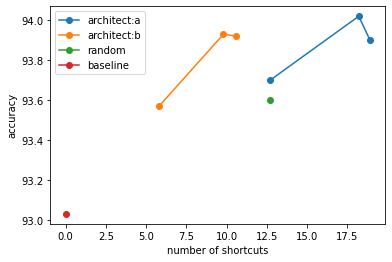
\includegraphics[clip,width=75mm]{short.png}
 		\caption{ショートカット数に対する精度}
 		\label{fig:short}
 	\end{center}
 \end{minipage}
\end{figure*}


\section{考察}
ランダムアーキテクチャの試行回数を増やして, 図\ref{fig:param}, \ref{fig:short}に
プロットすれば, 探索の効果がより分かりやすくなると思われる.

VGG19の事前学習モデルを利用することで近似の精度が上がり,
より有望な$\alpha$の探索ができると考えた.
ファインチューニングの動作確認もできたので,
\begin{itemize}
  \item 通常の探索時の初期重み
  \item GAでの探索時の初期重み
\end{itemize}
などの実験に使いたい.

\section{実験:猫}
224x224x3の猫データセット500枚を共有してもらったので,
CIFAR10以外のデータセットへの適用を考えた.

\subsection{問題}
Google Colabで開発していて水曜日までは動作していたコードが木曜日に動かなくなった?.
(内部の環境がアップデートされた?)
バグの修正方法を調査中.

\begin{table*}[t]
\begin{lstlisting}[caption=error code,label=code]
def normalized_alpha(self):
    alpha = torch.zeros_like(self.alphas[0])
    if self.evaluate:
      ...
    else:
      alpha[self.mask_f] = 1.0
      for a, raw, mask, b in zip(alpha, self.alpha(), self.mask_s, self.normalized_beta()):
        a[mask] = b * F.softmax(raw[mask], dim=0)
    return alpha

RuntimeError: Output 0 of a function created in no_grad mode is a view and is being modified inplace but this inplace operation is not allowed. You should either replace it by an out of place operation or do a .clone() of the Tensor before modifying it inplace. Note that this can happen when using DataParallel or DistributedDataParallel, which can send views of the original input to the forward method of the model.
\end{lstlisting}
\end{table*}


\section{今後の予定}
% なんとなくなんかの勉強をするとかではなく具体的に

\begin{itemize}
  % \item ランダムアーキテクチャとの比較
  % \item DARTのunrolling実験]
  % \item 閾値方式での評価
  \item バグの修正
  \item できればGAの実装
  \item 論文の調査
\end{itemize}

\section{ソースコード}
% 埋め込みでもGitでもいいので参照できるように
githubのnotebookリポジトリ参照.

% 参考文献リスト
\bibliographystyle{unsrt}
\bibliography{ref}
\end{document}
